
\clearpage{}
\section{Constraint ordering and mutual recursion}
\label{inference:ordering}

Consider the following program:

\code{
	\mc{4}{$\kproject \ \iInt \ \kwhere$} \\
	& $\ieven \ i$	& $= \kif \ i == 0 \ \kthen \iTrue  \hspace{0.3ex} \kelse  \ (i-1) \odot \iodd$ \\
	& $\iodd \ i$	& $= \kif \ i == 0 \ \kthen \iFalse   \kelse \ (i-1) \odot \ieven$ \\
	\\
	\mc{4}{$main \ () = \iprint \ 5 \odot \iodd$}
}

This program defines two projections, then uses the second to determine whether 5 is odd. Now, although we can plainly see that these projection functions are mutually recursive, the inference algorithm does not know this \emph{a priori}. This point should be clearer when we desugar the program into the simplified language described in \S\ref{Inference:Language}


\code{
	\mc{4}{$\kproject \ \iInt :: \% \to * \ \kwith$} \\
	& $\ieven$	& $\sim \iintEven$	\\
	& $\iodd$	& $\sim \iintOdd$	\\
}

\vspace{-1em}
\code{
	$\klet$ & $\imain$	& $= \lambda x. \ \kcase \ x \ \kof \iUnit \to \iprint \ 5 \odot \iodd$ \\

		& $\iintEven$	& $= \lambda i_1. \ \kif \ i_1 == 0 \ 
						\kthen \ \iTrue  \ 
						\kelse \ (i_1 - 1) \odot \iodd$ \\
		& $\iintOdd$	& $= \lambda i_2. \ \kif \ i_2 == 0 \ 
						\kthen \ \iFalse \ 
						\kelse \ (i_2 - 1) \odot \ieven$ \\
	$\kin$ 	& \dots
}

In this program we have introduced new bindings for each of the projection functions, expressed function bindings with $\lambda$-abstractions, added the kind signature for $\iInt$, and renamed the $i$ variables so they have unique names. We have also taken the liberty of moving the binding for $\imain$ to the front of the list, as it will make for a better example. Note that the projection labels $\ieven$ and $\iodd$ are not specific to the $\iintEven$ and $\iintOdd$ instance functions. We could have easily reused these labels in projection dictionaries for other types, so the inferencer really does need to infer that $(i_1 - 1)$ is an $\iInt$ before it can decide that $(i_1 - 1) \odot \ieven$ is implemented by $\iintEven$. 

This section gives an overview of how our type inference algorithm handles programs such as this one, that define recursive projections. The main point is that we must compute the binding dependency graph on the fly while we are inferring the types of expressions. We must also reorder bindings on the fly, so that the type of $\iintOdd$ will be known when we come to resolve the $5 \odot \iodd$ projection in the $\imain$ function.

The constraint tree for this program is shown on the following page, leaving out the constraints that aren't important to the discussion.

\clearpage{}
\begin{tabbing}
MMMM \=	MM \= MM \= MM \= MM \= MM \= MM \kill
 \>	GROUP \ $\{ \imain, \ \iintEven, \ \iintOdd \}$ \\
 \>	\> LET $\imain$ \\
 \>	\>	\> LAMBDA $x$ \\
 \>	\>	\>	\> $s_1$ \> $= \rPROJ \ \iodd \ s_2$ \\
 \>	\>	\>	\> $s_2$ \> $= \iInt \ r_1$ \\
 \>	\>	\> 	\> $\dots$ \\
 \>	\> LET $\iintEven$ \\
 \>	\>	\> LAMBDA $i_1$ \\
 \>	\>	\>	\> $s_3$ \> $= \rINST \ i_1$ \\
 \>	\>	\>	\> \dots \\
 \>	\>	\> 	\> $s_4$ \> $= \rPROJ \ \iodd \ s_5$ \\
 \>	\>	\>	\> $s_5$ \> $= \dots$ \\
 \>	\> LET $\iintOdd$ \\
 \>	\>	\> LAMBDA $i_2$ \\
 \>	\>	\>	\> $s_6$ \> $= \rINST \ i_2$ \\
 \>	\>	\>	\> \dots \\
 \>	\>	\> 	\> $s_7$ \> $= \rPROJ \ \ieven \ s_8$ \\
 \>	\>	\>	\> $s_8$ \> $= \dots$
\end{tabbing}

For the remainder of this section we will draw our constraint trees graphically, as it makes the presentation clearer. The above tree becomes:
\begin{center}
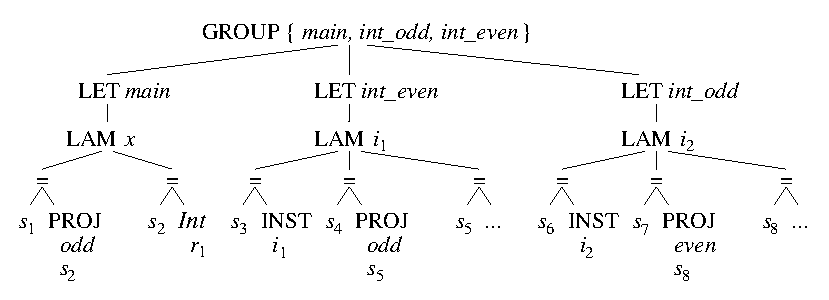
\includegraphics{3-Inference/fig/ordering/tree-start}
\end{center}

During type inference we perform a left to right, depth first traversal over the constraint tree. As we do this we delete constraints from the tree and add them to the type graph.  We start with a full tree and an empty type graph, and finish with a empty tree and a full graph. Internal nodes such as GROUP, LET and LAM organise the type constraints and represent the structure of the original program. We refer to the sub-tree headed by a GROUP, LET or LAM node as a GROUP, LET or LAM \emph{branch}. Once we have added all the constraints in a particular branch to the type graph we can delete the head-node as well. Deleting a LET node also triggers type generalisation, which we will discuss in a moment. Firstly, note that we when we arrive at an INST node, we can determine how the contained variable was bound by examining its parents. In the above example, we see that $i_1$ is lambda bound. In our practical implementation we maintain a stack of internal nodes for this purpose, pushing them onto the stack as we enter a branch, and popping as we leave.

As mentioned earlier, deletion of a LET node invokes generalisation of the type of the contained variable. However, recall from \S\ref{inference:generalisation} that before we generalise a type from the graph we must pack it into flat form, and this is only possible when the graph is in normal form. The graph is in normal form when no further reduction rules apply, and when it contains no unresolved PROJ or INST constraints. These two requirements ensure that we have solved all the constraints from a particular binding before we generalise its type. 

When performing type inference on a program whose bindings are not in dependency order, or whose bindings are mutually recursive, there will be situations when we wish to leave a LET branch but the graph is not in normal form. This will be because we have no type scheme to satisfy an INST node, or no type constructor to guide the reduction of a PROJ node. In these situations we remove the offending node from the graph and place it back in the tree, then restructure the tree so that further progress can be made before we need to perform the generalisation. This gives us time to infer the required type scheme, or determine the required type constructor, before we have to generalise the original type.

Both of these situations arise when typing the even/odd example on the previous page, so we will work through it now. We use $\bullet$ to indicate where we are in the traversal, and $\varepsilon$ to represent an empty branch. After descending into the right most branch and adding the $s_1$ and $s_2$ constraints we arrive at:

\begin{center}
\includegraphics{3-Inference/fig/ordering/tree-main-gen}
\end{center}
\vspace{-2em}
The type graph is:
\begin{tabbing}
MMMMM	\= MM 	\= MM 		\= MMMMMM 	\= MM \kill
	\> *1	\> $\sim$	\> $s_1$	\> $= \ \rPROJ \ \iodd \ s_2$ \\
	\> *2	\> $\sim$	\> $s_2$	\> $= \ \iInt \ r_1$
\end{tabbing}
Now, we would like to leave the current branch and generalise the type of $\imain$, but before we do that we must reduce the graph to normal form. This requires that we resolve the projection constraint in *1. The projection constraint refers to $s_2$, which is constrained to be $\iInt \ r_1$. This means that we can look up the instance function to use from the corresponding dictionary. Here is the $\iInt$ dictionary again:

\code{
	\mc{4}{$\kproject \ \iInt :: \% \to * \ \kwith$} \\
	& $\ieven$	& $\sim \iintEven$	\\
	& $\iodd$	& $\sim \iintOdd$	\\
}

The $\iodd$ instance for integers is $\iintOdd$, so we can crush the $\rPROJ$ node in the graph into an $\rINST$ of this function's type. This yields:
\begin{tabbing}
MMMMM	\= MM 	\= MM 		\= MMMMMM 	\= MM \kill
	\> *1	\> $\sim$	\> $s_1$	\> $= \ \rINST \ \iintOdd$ \\
	\> *2	\> $\sim$	\> $s_2$	\> $= \ \iInt \ r_1$
\end{tabbing}

Now, we cannot actually instantiate the type for $\iintOdd$ yet because we haven't inferred it. Instead, we will defer further work on the type of $\imain$ and focus on $\iintOdd$ instead. We do this by removing the $s_1 = \ \rINST \ \iintOdd$ constraint from the graph and placing it back in the tree. We then move the LET $\iintOdd$ branch under LET $\imain$, so we can work on that before returning to generalise the type of $\imain$:
\begin{center}
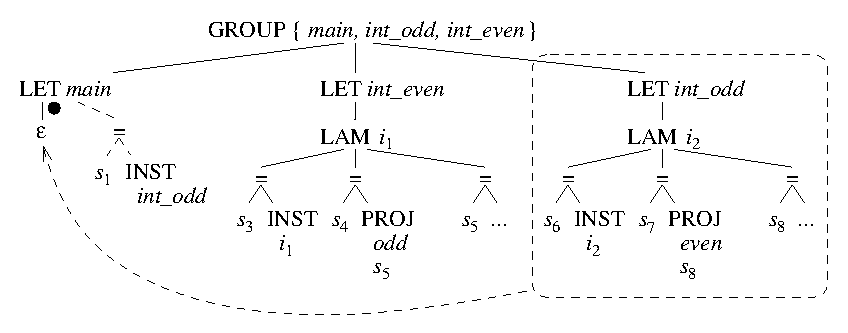
\includegraphics{3-Inference/fig/ordering/tree-main-gen-move}
\end{center}
Note that the $s_1 = \ \rINST \ \iintOdd$ constraint is placed \emph{after} the LET branch, so that the type for $\iintOdd$ will have been generalised before we need to instantiate it. Completing the move yields:
\begin{center}
\includegraphics{3-Inference/fig/ordering/tree-main-gen-moved}
\end{center}

We can now continue our depth first traversal into the $\iintOdd$ branch, adding the constraints for $s_6$, $s_7$ and $s_8$ to the type graph. Assuming $s_8$ resolves to the type $\iInt \ r_2$, we end up with the following graph:
\begin{tabbing}
MMMMM	\= MM 	\= MM 		\= MMMMMM 	\= MM \kill
	\> *1	\> $\sim$	\> $s_1$	\> $= \ \bot$ \\
	\> *2	\> $\sim$	\> $s_2$	\> $= \ \iInt  \ r_1$ \\
	\> *3	\> $\sim$	\> $s_6$	\> $= \ s_{i_2}$ \\
	\> *4	\> $\sim$	\> $s_7$	\> $= \ \rPROJ \ \ieven \ s_8$ \\
	\> *5	\> $\sim$	\> $s_8$	\> $= \ \iInt \ r_2$
\end{tabbing}

Note that in our constraint tree, the constraint $s_6 = \rINST \ i_2$ appears under the $\rLAM \ i_2$ node, which tells us that $i_2$ is lambda bound. As we do not support higher rank types, lambda bound variables do not have polytypes. This means that we do not have to instantiate them, and we can simplify the $s_6$ constraint to $s_6 = s_{i_2}$. 

\clearpage{}
After the constraints from the $\iintOdd$ branch are added, our constraint tree is:
\begin{center}
\includegraphics{3-Inference/fig/ordering/tree-intodd-gen}
\end{center}
\vspace{-2em}
And the graph is still:
\begin{tabbing}
MMMMM	\= MM 	\= MM 		\= MMMMMM 	\= MM \kill
	\> *1	\> $\sim$	\> $s_1$	\> $= \ \bot$ \\
	\> *2	\> $\sim$	\> $s_2$	\> $= \ \iInt  \ r_1$ \\
	\> *3	\> $\sim$	\> $s_6$	\> $= \ s_{i_2}$ \\
	\> *4	\> $\sim$	\> $s_7$	\> $= \ \rPROJ \ \ieven \ s_8$ \\
	\> *5	\> $\sim$	\> $s_8$	\> $= \ \iInt \ r_2$
\end{tabbing}

Now, the $\bullet$ shows that we are still inside the $\rLET \iintOdd$ branch. However, we cannot leave it yet and generalise the type of $\iintOdd$ because the graph contains an unresolved PROJ constraint, so is not in normal form. As before, this constraint refers to $s_8$ which an $\iInt$, so we can lookup the projection instance function from the corresponding dictionary and crush $\rPROJ \ \ieven \ s_8$ to $\rINST \ \iintEven$. Note that crushing a $\rPROJ$ constraint in this way corresponds to discovering part of the program's call tree, because we now know that $\iintOdd$ calls $\iintEven$. The new graph is:
\begin{tabbing}
MMMMM	\= MM 	\= MM 		\= MMMMMM 	\= MM \kill
	\> *1	\> $\sim$	\> $s_1$	\> $= \ \bot$ \\
	\> *2	\> $\sim$	\> $s_2$	\> $= \ \iInt  \ r_1$ \\
	\> *3	\> $\sim$	\> $s_6$	\> $= \ s_{i_2}$ \\
	\> *4	\> $\sim$	\> $s_7$	\> $= \ \rINST \ \iintEven$ \\
	\> *5	\> $\sim$	\> $s_8$	\> $= \ \iInt \ r_2$
\end{tabbing}
We still cannot generalise the type of $\iintOdd$ since it is not in normal form. As before, we will remove the offending $s_7 = \ \rINST \ \iintEven$ constraint from the graph and place it back in the tree, then reorganise the tree so we can make further progress. This gives:

\begin{center}
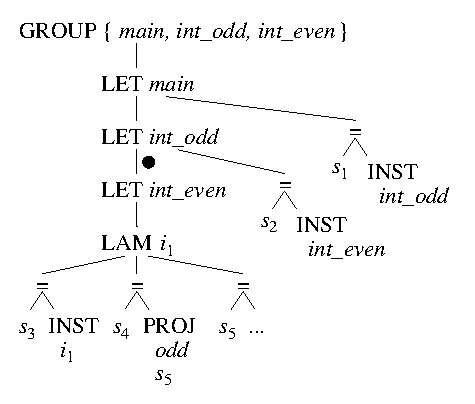
\includegraphics{3-Inference/fig/ordering/tree-intodd-gen-moved}
\end{center}

\clearpage{}
\begin{center}
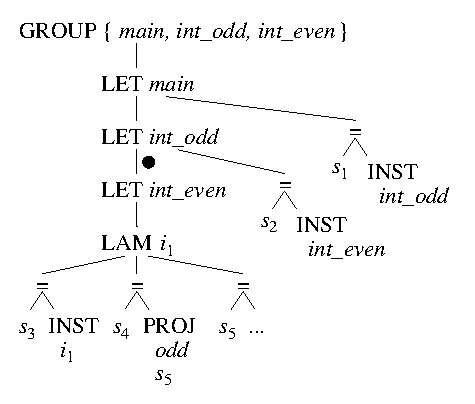
\includegraphics{3-Inference/fig/ordering/tree-intodd-gen-moved}
\end{center}
\vspace{-1em}
As before, we can continue our traversal by descending into the left of the tree, and adding the constraints for $s_3$, $s_4$ and $s_5$ to the graph. Once this is done we have:
\begin{center}
\includegraphics{3-Inference/fig/ordering/tree-inteven-gen}
\end{center}
After crushing the $s_4 = \rPROJ \ \iodd \ s_5$ constraint to $s_4 = \rINST \ \iintOdd$ the type graph becomes:
\begin{tabbing}
MMMMM	\= MM 	\= MM 		\= MMMMMM 	\= MM \kill
	\> *1	\> $\sim$	\> $s_1$	\> $= \ \bot$ \\
	\> *2	\> $\sim$	\> $s_2$	\> $= \ \iInt  \ r_1$ \\
	\> *3	\> $\sim$	\> $s_6$	\> $= \ s_{i_2}$ \\
	\> *4	\> $\sim$	\> $s_7$	\> $= \ \bot$ \\
	\> *5	\> $\sim$	\> $s_8$	\> $= \ \iInt \ r_8$ \\
	\> *6	\> $\sim$	\> $s_3$	\> $= \ s_{i_1}$ \\
	\> *7	\> $\sim$	\> $s_4$	\> $= \ \rINST \ \iintOdd$ \\
	\> *8	\> $\sim$	\> $s_5$	\> $= \ \iInt \ r_5$ 
\end{tabbing}
Note that at this point, we have discovered that $\iintOdd$ and $\iintEven$ are mutually recursive. This becomes clear when we place $s_4 = \ \rINST \ \iintOdd$ back in the tree:
\begin{center}
\includegraphics{3-Inference/fig/ordering/tree-inteven-moved}
\end{center}

\clearpage{}
In this tree, the fact that the $\rINST \ \iintOdd$ constraint appears under $\rLET \ \iintEven$ tells us that the binding for $\iintEven$ references $\iintOdd$, likewise, $\iintOdd$ references $\iintEven$. As with Haskell \cite{jones:typing-haskell}, in the absence of polymorphic recursion we type mutually recursive bindings using monotypes for the bound variables. This allows us to rewrite the $s_4 = \rINST \ \iintOdd$ and $s_2 = \rINST \ \iintEven$ constraints to $s_4 = s_{\iintOdd}$ and $s_2 = s_{\iintEven}$. These can be added directly to the graph without needing to instantiate type schemes for $\iintOdd$ or $\iintEven$. Note that in this example we have elided the majority of the constraints from the program. In practice, after adding the two constraints $s_4 = s_{\iintOdd}$ and $s_2 = s_{\iintEven}$ we will need to perform unifications and other reductions to return it to normal form. 

Finally, when leaving the $\rLET \ \iintEven$ and $\rLET \ \iintOdd$ branches, we must wait until we are outside all the branches of a binding group before we generalise their types. This ensures that all constraints from all bindings in the group have been processed, and that we treat the group as a single unit. 



\subsection{Comparison with Helium. 2002 -- \\
 Heeren, Hage, Swierstra.}
There are many degrees of freedom to the order in which constraints are processed. If a program contains multiple type errors, then solving constraints in a different order affects which errors are encountered first. For all other programs, changing the order should not affect the substance of the solution.

However, there \emph{is} one overriding restriction. Before the type of a let-bound variable can be generalised into a type scheme, all the constraints from the right of the binding must have been added to the graph. If we fail to do this then the resulting scheme may be instantiated at several different types before we encounter a constraint that would have prevented part of it from being generalised. 

We handle this restriction by expressing the type constraints as a tree. Each let-binding corresponds to a branch in the tree, and during our traversal we use the structure of the tree to ensure that constraints from sub-branches are added to the graph before the type of the binding is generalised. In contrast, in the Helium~\cite{heeren:constraint-type-inferencing, heeren:generalising-hm} compiler, the type constraints fed to the solver have a flat structure, and the requirement to process constraints from the right of a let-binding before generalising the type of the bound variable is handled in a different way.

Helium uses a constraint of the following form: 

\code{
	$\tau_1 \leq_M \tau_2$
}

This constraint says that $\tau_1$ is obtained by first generalising $\tau_2$ with respect to the set of monomorphic variables $M$, and then instantiating the resulting type scheme. The restriction is enforced by requiring that all constraints involving type variables that are present in $\tau_2$, but cannot appear in $M$, are processed first. This requirement ensures that the form of $\tau_2$ cannot change once we make the type scheme. We feel that this is a more elegant solution than our own method of dynamically reordering constraint trees. 

On the other hand we are unsure whether it is possible to adapt Helium's algorithm to deal with the mutually recursive projection definitions considered in this section. In \cite{heeren:constraint-type-inferencing}, the rules given to extract type constraints from the source program require the calculation of the binding dependency graph, and we have seen that this is not possible with recursive projections. It would seem that to calculate the binding dependency graph on the fly, we must retain information about which projections appear in which bindings. It may well be possible to construct a hybrid of Helium's system and our own, but we have not looked into it in detail.

We also wonder about the run time cost of determining which of the $\tau_1 \leq_M \tau_2$ constraints in the graph are ready to be processed. Using a flat constraint tree provides more freedom to choose the order in which constraints are considered, but using a hierarchical one provides more direction. Chapter 4 of \cite{heeren:top-quality-error-messages} contains further discussion of the pros and cons of several related approaches.

Besides the restriction outlined above, it is also important that enough type information makes it into the graph before we are forced to resolve projection constraints. In our current implementation, a particular type is only generalised the first time we need to instantiate it. If there are no bound occurrences of a variable in the module being compiled, which is common for library code, then its type is generalised after all other information is added to the graph. We are unsure whether our chosen approach admits edge cases where a particular projection constraint ``should have'' been resolved, but wasn't. This would create spurious ambiguous projection errors, but we have not noticed any so far.




 



